\documentclass[11pt,a4paper]{article}
\usepackage[a4paper,margin=2.3cm]{geometry}
\usepackage{amsmath,amssymb,amsthm}
\usepackage{booktabs}
\usepackage{graphicx}
\usepackage{float}
\usepackage[numbers]{natbib}
\usepackage{hyperref}
\usepackage{xcolor}
\usepackage{enumitem}
\usepackage{array}
\usepackage{longtable}
\usepackage{caption}
\graphicspath{{figures/}{figures/peak_shaving_diagnostics/}{figures/peak_shaving_submission/}{figures/peak_shaving_smpt/}{./}}
\hypersetup{colorlinks=true,linkcolor=blue,citecolor=blue,urlcolor=blue}
\captionsetup{font=small}
\setlength{\emergencystretch}{3em}

\newtheorem{proposition}{Proposition}
\newtheorem{remark}{Remark}
\newtheorem{assumption}{Assumption}
\newtheorem{definition}{Definition}
\newcommand{\qos}{q}
\newcommand{\T}{\mathcal{T}}
\newcommand{\M}{\mathcal{M}}
\newcommand{\D}{D}
\newcommand{\w}{\boldsymbol{w}}
\newcommand{\p}{\boldsymbol{p}}
\newcommand{\g}{\boldsymbol{g}}

\title{\textbf{A Simulation-Based Study of Time-of-Use Pricing for Fixed-Capacity AI Inference Services:\\
QoS Protection and the Profit Boundary}}
\author{Anonymous Author}
\date{}

\begin{document}
\maketitle

\begin{abstract}
Fixed-capacity AI inference services face daily load variation: peak periods degrade latency and completions, while off-peak GPUs remain costly. This paper develops an auditable simulation model for studying time-of-use pricing in an inference-service market with two heterogeneous providers, an API intermediary, direct-provider channels, time-rigid and time-flexible users, QoS feedback, and outside-option exit. The model is implemented as a candidate-response simulation over a low-dimensional price-shape family, with fictitious play, fixed-point QoS routing, and finite-grid regret diagnostics used to make solver limits explicit. In the congested synthetic setting, uniform pricing gives peak utilization $0.782$ and minimum QoS $0.756$. Dynamic coarse and fine candidate responses reduce peak utilization to $0.706$ and $0.666$ and increase minimum QoS to $0.968$ and $0.990$. A double-oracle mixed-strategy diagnostic on the full 225-point grid obtains maximum regret $0.203$, expected peak utilization $0.703$, and minimum QoS $0.970$. Local fixed-policy perturbations across capacity, price sensitivity, switching cost, and the QoS threshold preserve QoS gains and peak-utilization reductions. Profit is not robust: the coarse response gives $+9.3\%$, the fine response $-1.9\%$, and the mixed profile about $-2.8\%$. The results position time-of-use pricing as a QoS-protection mechanism under fixed capacity, not as a reliable profit-improvement rule. Public API prices and controlled vLLM measurements are used only as scale and QoS-shape anchors; the economic calibration remains synthetic.
\end{abstract}

\noindent\textbf{Keywords:} simulation modelling; inference service; dynamic pricing; QoS; peak shaving; finite-grid regret; sensitivity analysis

\section{Introduction}
\label{sec:intro}

Large-model inference has moved from offline batch jobs to continuously running online services. Chat, code generation, agent workflows, periodic evaluation, and scheduled batch tasks arrive at different times of day. GPU inference clusters face load peaks that are not easy to remove by short-run capacity expansion \cite{crankshaw2017clipper,gujarati2020clockwork,yu2022orca,kwon2023pagedattention,agrawal2024sarathiserve}. When utilization approaches a local capacity threshold, time-to-first-token latency, queueing delay, and completion rates can deteriorate quickly. Lower service quality then reduces the volume of requests that can be completed and billed.

This paper focuses on a fixed-capacity setting. GPU procurement and deployment have lead times and sunk costs, and idle off-peak GPUs still carry holding costs. A natural response is to use prices rather than capacity expansion: charge more in peak periods, charge less off peak, and move time-flexible demand where the system has spare capacity. This idea is close in spirit to real-time electricity pricing and demand response \cite{schweppe1988spot,borenstein2005long,albadi2008summary,faruqui2010household,siano2014demand}. The engineering object is different. Inference-service quality is governed by local GPU utilization, latency, and completion rates rather than generation constraints or power-flow equations.

Inference markets also differ from the single-platform monopoly often used in simple pricing models. The same open-source model family, such as GLM, can be deployed by more than one provider. If the user-visible model capability is similar, competition turns on price, available capacity, and realized QoS. Provider capacity is also uneven. A smaller provider can enter congestion sooner when an intermediary routes traffic to it. These observations motivate a two-provider model with heterogeneous fixed capacities, one API intermediary that routes traffic between providers, and users who may also buy directly from providers or leave the market.

The simulation study is organized around three questions:
\begin{enumerate}[label=\textbf{RQ\arabic*.},leftmargin=2.8em]
  \item Under fixed GPU serving capacity, can time-of-use pricing reduce peak utilization and protect the worst-period QoS?
  \item Which modelling components make the QoS result appear: time flexibility, provider heterogeneity, direct-provider channels, outside-option exit, or QoS-aware routing?
  \item Does the same mechanism also produce a reliable profit gain, or does it mainly reallocate surplus and congestion loss?
\end{enumerate}

The paper contributes a reproducible simulation workflow rather than a closed-form equilibrium theory. First, it gives a fixed-capacity model of time-of-use inference pricing with two competing providers, one routing intermediary, time-rigid and time-flexible users, and an outside option. Second, it uses a low-dimensional pricing-shape family and fictitious play to obtain reproducible candidate responses, while reporting regret where the solver has not reached a strong equilibrium certificate. Third, it separates the QoS result from the profit result. The experiments support a finite-grid QoS-protection claim in the congested setting, but they do not support a reliable profit-improvement claim.

\section{Related Work and Positioning}
\label{sec:related}

The paper is positioned between three literatures. Systems work on inference serving explains why batching, memory management, and scheduling affect latency and throughput \cite{crankshaw2017clipper,gujarati2020clockwork,romero2021infaas,yu2022orca,li2023alpaserve,sheng2023flexgen,kwon2023pagedattention,agrawal2024sarathiserve,patel2024splitwise,zhong2024distserve,agrawal2024vidur}. This line of work usually treats the request set as given and does not put prices, outside options, and cross-provider competition in the same market model. Congestion pricing and revenue management study how prices allocate scarce capacity under time-varying demand \cite{vickrey1969congestion,arnott1990bottleneck,gallego1994dynamic,elmaghraby2003dynamic,bitran2003overview,talluri2004revenue,phillips2005pricing}. Recent work on AI-service markets has begun to discuss inference costs, menu pricing, token-capacity contracts, and Stackelberg-style pricing for GPU services \cite{demirer2025emerging,erdil2025inference,bergemann2025menu,guo2026prillm,yan2026stackelberg,cunningham2026token,liu2026locational}. User choice follows standard discrete-choice and platform-market tools \cite{mcfadden1974conditional,anderson1992discrete,train2009discrete,rochet2003platform}.

The gap addressed here is therefore methodological and application-specific. We do not propose a new serving scheduler, a new revenue-management theorem, or a production demand forecast. The contribution is a transparent simulation model that puts QoS congestion, provider heterogeneity, intermediary routing, direct-provider alternatives, and market exit in the same fixed-capacity experiment, then reports where the numerical evidence is strong and where it is not.

\section{Conceptual Simulation Model}
\label{sec:model}

The conceptual model abstracts one inference-service day into interacting price, routing, demand, load, QoS, and profit components. It is not intended to be a digital twin of a specific provider. The purpose is to keep enough structure to trace how a price-shape change moves demand across time and channels, while keeping the implementation small enough for artifact-level verification.

\subsection{Market structure}

A day is divided into $T$ periods, $\T=\{1,\ldots,T\}$, each of length $h$. The market contains two inference providers, $\M=\{A,B\}$, with fixed capacities $G_A>G_B$. Both deploy the same open-source model and are treated as nearly homogeneous in model quality. Provider $m$ posts a period-specific wholesale price $w_{m,t}$ to the intermediary and a direct retail price $p^D_{m,t}$ to users.

The API intermediary observes wholesale prices and chooses a retail price $p_t$ and routing weights $r_{m,t}$, with $\sum_m r_{m,t}=1$. Users choose among the intermediary channel, direct access to provider $A$, direct access to provider $B$, and an outside option. The timing is: providers post prices, the intermediary responds, users choose channels and periods, and a QoS congestion fixed point maps demand into effective service.

\begin{figure}[H]
\centering
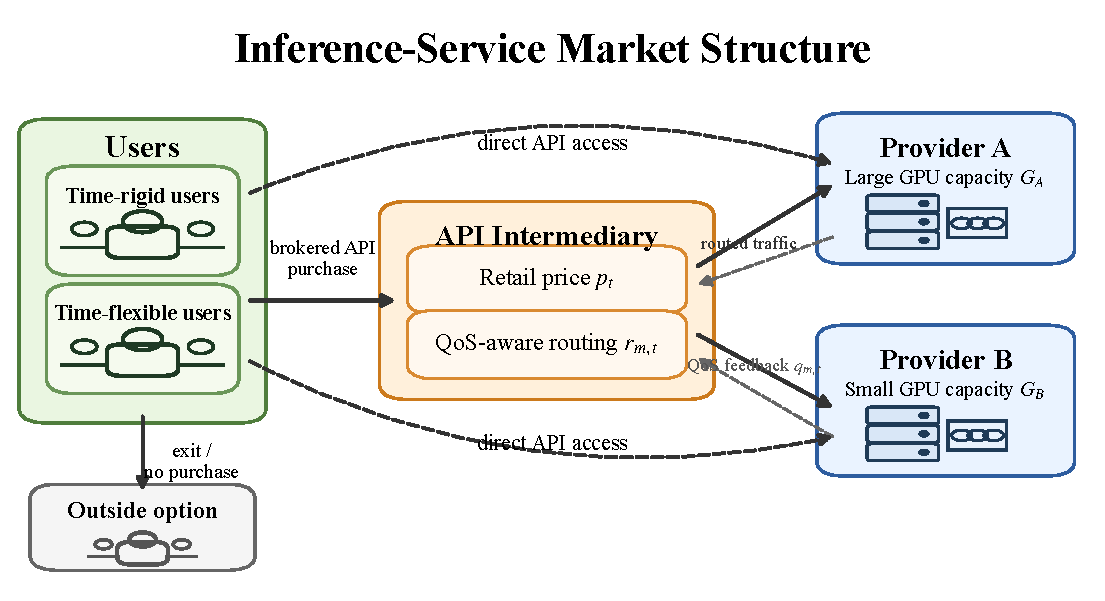
\includegraphics[width=0.82\textwidth]{market_schematic.pdf}
\caption{Market structure. Users can buy through the API intermediary, connect directly to a provider, or exit. The intermediary routes traffic between two providers based on prices and QoS.}
\label{fig:market_schematic}
\end{figure}

\subsection{User choice and outside option}

There are two user types, $\theta\in\{R,E\}$. Type $R$ users are time-rigid; type $E$ users are time-flexible. For channel $k$ and period $t$, deterministic utility is
\begin{equation}
  z^\theta_{k,t}=\log b_k+\log a_t
  -\alpha_\theta\!\left[\text{price}_{k,t}+c_s^\theta(1-\pi^\theta_t)-p_0\right]
  -\gamma(1-q_{k,t}).
  \label{eq:utility}
\end{equation}
Here $b_k$ is channel convenience, $a_t$ is period preference, $\pi^\theta_t$ is the native-period distribution, and $q_{k,t}$ is channel QoS. Switching cost is expressed in price-equivalent units and is scaled by the same price-sensitivity parameter $\alpha_\theta$. Time-rigid users have lower price sensitivity, higher switching cost, and a more peaked native-period distribution.

The logit denominator includes a no-purchase outside option with utility $u_0$:
\begin{equation}
  s^\theta_{k,t}=\frac{\exp(z^\theta_{k,t})}{\exp(u_0)+\sum_{k',t'}\exp(z^\theta_{k',t'})},
  \qquad
  s^\theta_0=\frac{\exp(u_0)}{\exp(u_0)+\sum_{k',t'}\exp(z^\theta_{k',t'})}.
  \label{eq:share}
\end{equation}
The outside share is not redistributed to the inside options. When prices rise, some demand leaves the market rather than being mechanically reallocated to another channel.

\subsection{Demand, load, and QoS}

Demand combines a flexible market-size term and a rigid replay term:
\begin{equation}
  \D^\theta_{k,t}=\bar F_\theta\,m(\p)\,s^\theta_{k,t}
  +\bar R^\theta_t\,\sigma[\beta(v_r-\text{price}_{k,t})]\,s^\theta_{k,t}.
  \label{eq:demand}
\end{equation}
Total demand is the population-weighted sum of the two types. The model is not a fixed-total-demand model. The outside option allows internal demand to shrink, and the flexible market-size term allows lower prices to expand demand. Later profit interpretations should be read as numerical mechanism analysis, not as a theorem under fixed total demand.

Provider $m$'s load in period $t$ is direct demand plus intermediary traffic:
\begin{equation}
  L_{m,t}=\D^D_{m,t}+r_{m,t}\,\D^I_t,\qquad
  u_{m,t}=L_{m,t}/G_m,\qquad q_{m,t}=\qos(u_{m,t}).
  \label{eq:load}
\end{equation}
The QoS function begins to decline once utilization exceeds a threshold $\bar u$. Since $G_B<G_A$, the smaller provider reaches the congestion region earlier under the same incoming load. The main experiments use a smooth sigmoid-type degradation function. Threshold, linear, and square-root variants are used as robustness checks in the existing artifact set.

\subsection{Profit}

Provider profit is wholesale revenue plus direct retail revenue, minus fixed capacity holding cost and QoS degradation cost:
\begin{equation}
  \Pi_m=h\!\sum_t\! w_{m,t}r_{m,t}\D^I_t q_{m,t}
  +h\!\sum_t\! p^D_{m,t}\D^D_{m,t}q_{m,t}
  -h\!\sum_t\! c_g G_m
  -h\!\sum_t\! c_q(1-q_{m,t})L_{m,t}.
  \label{eq:firm_profit}
\end{equation}
The holding cost $c_gG_m$ is charged on fixed capacity, not on realized utilization. It gives providers a reason to fill off-peak capacity. Intermediary profit is retail revenue minus wholesale cost and QoS degradation cost. System profit is the sum of provider profits and intermediary profit.

\section{Computational Implementation and Candidate-Response Solver}
\label{sec:solver}

The computational model follows the equations in Section~\ref{sec:model} with deterministic candidate evaluation. Each strategy candidate is converted into period prices, the intermediary solves a routing and retail-pricing response, and a damped QoS fixed point maps routed demand into provider utilization and effective service. This section describes the search restriction and the diagnostics used to keep the solver boundary visible.

\subsection{Pricing-shape family}

Directly optimizing $2T$ continuous prices for each provider would create a high-dimensional, non-convex game with weak reproducibility. We instead restrict provider prices to a low-dimensional time-shape family:
\begin{equation}
  w_{m,t}=\bar w_m\big(1+\delta_m\,\widehat{\ell}_t\big),\qquad
  p^D_{m,t}=\bar p^D_m\big(1+\delta^D_m\,\widehat{\ell}_t\big).
  \label{eq:shape}
\end{equation}
The vector $\widehat{\ell}_t$ is a zero-mean normalized load shape derived from the rigid-demand baseline. Each provider strategy is represented by four scalars, $(\bar w_m,\delta_m,\bar p^D_m,\delta^D_m)$. A value of $\delta_m=0$ gives uniform pricing; $\delta_m>0$ raises peak-period prices. This restriction trades global optimality for transparency and repeatability. All equilibrium language in this paper refers to this finite shape family unless stated otherwise.

\subsection{Fictitious play and regret reporting}

Provider best responses are computed by grid search over the four pricing-shape parameters. The intermediary response is also found by grid search; each candidate evaluation solves a damped fixed point for routing and QoS. This design is deliberately simple. It is slower than a smooth optimizer on easy instances, but it is less fragile around non-smooth QoS responses and makes the search budget explicit.

Naive best-response iteration cycles in the congested regime. The providers repeatedly switch between two configurations rather than settling. We use fictitious play: each provider responds to the opponent's running average strategy, not only to its latest move. The output is a time-averaged strategy within the pricing-shape family. We treat it as a useful equilibrium approximation only when unilateral deviation regret is low.

\begin{remark}[Solver boundary]
In the uncongested regime, QoS is always one and the fixed point converges in one step. Across random seeds, the relative standard deviation of system profit is $4.31\times10^{-4}$. The congested regime is more delicate. On the coarse grid, fictitious-play regret declines from $133.6$ to $4.98$ in 22 rounds. On the fine-grid pure snapshot, regret bottoms near $14$ around round 10 and later drifts to about $22$ by round 40. The double-oracle finite-grid mixed diagnostic obtains a $5\times5$ support profile with full-grid maximum regret $0.203$ on the complete 225-point grid. This supports a finite-grid mixed-strategy interpretation of the QoS result, but not a continuous-space equilibrium theorem.
\end{remark}

\section{Verification, Validation, and Credibility Boundaries}
\label{sec:vv}

The simulation is deterministic conditional on the reported grids, parameter settings, and solver seeds. Verification asks whether the code implements the accounting, routing, and fixed-point calculations used in the paper. Validation asks a narrower question: whether the abstractions are credible enough for a mechanism study of fixed-capacity inference pricing. The checks below are meant to bound the claims, not to certify a production service model.

\subsection{Implementation verification}

The implementation keeps the market equations, fixed-point QoS update, intermediary response, and provider candidate search in separate modules. The main verification checks are artifact based. The uncongested setting gives QoS equal to one and converges immediately, which is a sanity check that the degradation function is inactive below the utilization threshold. Cross-seed runs in this regime give relative standard deviation $4.31\times10^{-4}$ for system profit. In the congested setting, the reported artifacts record the baseline uniform profile, coarse and fine candidate responses, checkpoint traces, diagnostic figures, and mixed-strategy oracle output.

The fixed-point routine reports convergence flags and iteration counts for the evaluated market state. For the main SMPT diagnostic records, the static baseline and four dynamic-policy variants converge with final residuals below $10^{-9}$. The static baseline takes 52 iterations; off-peak-discount-only, peak-surcharge-only, dynamic coarse, and dynamic fine take 32, 34, 33, and 35 iterations, respectively. A small initialization and damping audit over three initial QoS levels and three damping factors gives convergence in 24 of 27 rows. The dynamic coarse and fine rows converge in all 18 combinations; the three non-converged rows occur for the static uniform baseline with damping $0.5$, where the residual remains about $0.312$ at the 200-iteration limit. These checks do not exhaust all candidate evaluations in the grid search, but they verify the fixed-point states used in the reported dynamic-policy comparisons and identify a real numerical boundary for the static congested case.

\subsection{Validation and calibration boundary}

The model is validated only in a limited, measurement-informed sense. Public API prices are used to check the scale of normalized price ranges, not to estimate user demand elasticity. Controlled vLLM overload scans are used to anchor the shape of the QoS degradation curve: QoS remains close to one below a healthy concurrency point and declines beyond it. These scans use one GPU, two small model profiles, short generations, five repeats per concurrency level, and a single time-to-first-token SLA threshold. They support the qualitative threshold-shaped QoS assumption, but they do not validate a production inference service or a real platform market.

The sensitivity evidence is reported in three layers. First, a fixed-policy stress test perturbs capacity, price sensitivity, switching cost, and the QoS threshold. Second, a two-dimensional fixed-policy phase grid varies capacity scale and price-sensitivity scale. Third, a restricted local candidate re-solve is run for five selected perturbations. The last layer uses a small local candidate set built from static, dynamic coarse, dynamic fine, off-peak-only, and peak-only shapes; it is a re-solved simulation diagnostic, not a global equilibrium computation.

\section{Experimental Design}
\label{sec:setup}

The horizon has $T=8$ periods and $h=3$ hours per period. Baseline capacity is $G_A=1500,G_B=600$. The congested setting tightens capacity to $G_A=300,G_B=120$. Baseline population weights are $(\pi_R,\pi_E)=(0.6,0.4)$; the congested setting uses $(0.4,0.6)$ to increase peak pressure. All economic parameters are synthetic calibrations used to study mechanism direction, not production forecasts.

The experimental design has four evidence layers. The first compares uniform pricing with dynamic candidate responses in uncongested and congested regimes. The second reports solver diagnostics, including pure-strategy regret and the finite-grid mixed oracle. The third adds service-management baselines and structural ablations. The fourth uses fixed-policy stress tests, a capacity--elasticity phase grid, and restricted local re-solves. The main output measures are peak utilization, minimum QoS, served volume, system profit, exit probabilities, and regret. This design lets the paper test the QoS mechanism without treating every profit change as a robust finding.

We use public API prices only as scale checks. The verified public prices are: Z.AI GLM-4.7 at \$0.6 per million input tokens and \$2.2 per million output tokens; DeepSeek-chat at \$0.27 cache-miss input and \$1.10 output; and OpenAI GPT-4o at \$2.50 input and \$10.00 output \cite{zaiPricing2026,deepseekPricing2026,openaiGpt4oPricing2026}. These values are not used to estimate user elasticity.

We also reuse two controlled vLLM single-GPU overload scans as QoS-shape anchors. The backend is vLLM 0.22.0 on an NVIDIA GeForce RTX 4090. The models are Qwen2.5-0.5B-Instruct and Qwen2.5-3B-Instruct. Each concurrency level is repeated five times. The observed QoS is the share of runs whose time to first token is at most 0.5 seconds. Both scans keep this SLA rate at one up to normalized concurrency one and then decline beyond the healthy concurrency point. Fitting $q(u)=\exp[-\kappa(u-\bar u)^2_+]$ gives $(\bar u,\kappa,\mathrm{RMSE})=(1.000,0.517,0.068)$ for the 0.5B profile and $(1.058,0.942,6.3\times10^{-10})$ for the 3B profile. This is a shape anchor, not a production SLA calibration.

\begin{figure}[H]
\centering
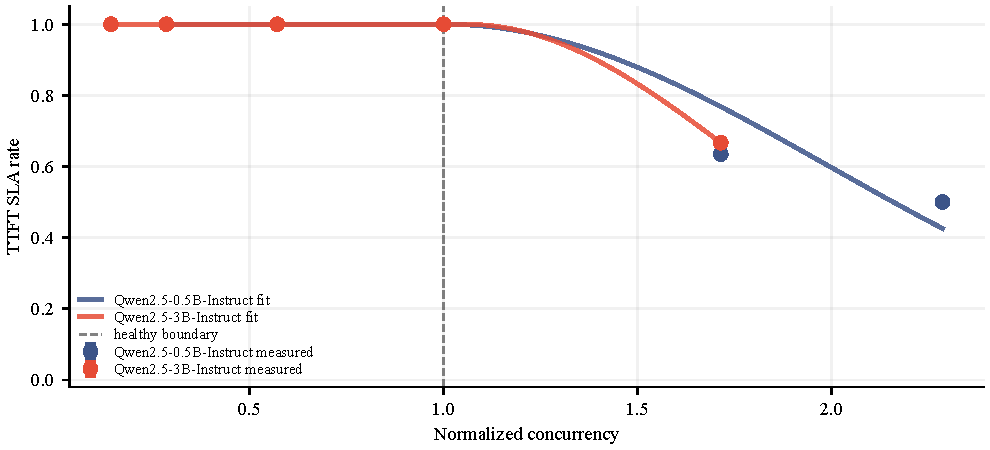
\includegraphics[width=0.88\textwidth]{vllm_qos_anchor.pdf}
\caption{Controlled vLLM single-GPU QoS-shape anchor. The x-axis is concurrency normalized by the largest healthy concurrency level. The y-axis is the SLA attainment rate for a 0.5-second time-to-first-token threshold. Points are means over five repeats; lines are fitted threshold-type QoS curves.}
\label{fig:vllm_qos_anchor}
\end{figure}

\section{Results}
\label{sec:results}

\subsection{Uncongested regime}

With baseline capacity, uniform pricing reaches only $0.213$ peak utilization and QoS remains one. Dynamic pricing still shifts demand, but it has little room to improve QoS.

\begin{table}[H]
\centering
\caption{Uncongested regime: uniform pricing and dynamic pricing}
\label{tab:uncongested}
\begin{tabular}{lcc}
\toprule
Metric & Uniform pricing & Dynamic pricing \\
\midrule
System profit & 1193.3 & 1139.4 \\
Peak utilization & 0.213 & 0.261 \\
Elastic-demand centroid shift & \multicolumn{2}{c}{$+0.177$} \\
Rigid-demand centroid shift & \multicolumn{2}{c}{$+0.077$} \\
\bottomrule
\end{tabular}
\end{table}

The demand-shift result is consistent with the model design. The time-flexible group shifts by about 2.3 times as much as the time-rigid group. Profit, however, is neutral to mildly negative in this regime. Across the elastic-population scan, gains are $0\%,-0.32\%,-4.51\%,-3.76\%,-3.00\%$. Dynamic pricing needs actual congestion before it can protect QoS.

\subsection{Congested regime}

Tightening capacity creates a genuine congested case under uniform pricing. Table~\ref{tab:congested} reports uniform pricing, the dynamic coarse-grid time-averaged strategy, the dynamic fine-grid pure snapshot, and the finite-grid mixed diagnostic.

\begin{table}[H]
\centering
\caption{Congested regime: uniform pricing and dynamic time-of-use pricing}
\label{tab:congested}
\small
\begin{tabular}{lcccc}
\toprule
Metric & Uniform & Dynamic coarse & Dynamic fine snapshot & Mixed diagnostic \\
\midrule
Peak utilization & 0.782 & 0.706 & 0.666 & 0.703 \\
Minimum QoS & 0.756 & 0.968 & 0.990 & 0.970 \\
System profit & 1783 & 1949 & 1749 & 1733 \\
Profit change & -- & $+9.3\%$ & $-1.9\%$ & $-2.8\%$ \\
Max regret & -- & 4.98 & 22.30 & 0.203 \\
\bottomrule
\end{tabular}
\end{table}

\begin{table}[H]
\centering
\caption{Evidence boundary for the congested regime}
\label{tab:evidence_boundary}
\small
\begin{tabular}{p{0.25\textwidth}p{0.31\textwidth}p{0.34\textwidth}}
\toprule
Object & Solver status & Claim allowed in this paper \\
\midrule
Uniform baseline & Fictitious play reaches the criterion within 10 rounds & Used as the congested baseline. \\
Dynamic coarse grid & Regret is $4.98$ after 22 rounds, but coarse resolution can hide finer deviations & Useful as a low-resolution diagnostic, not a standalone profit conclusion. \\
Dynamic fine snapshot & Max regret is about $22.3$ after 40 rounds & Used as a resolution stress snapshot, not as a pure-strategy equilibrium claim. \\
Finite-grid mixed diagnostic & Full 225-point grid max regret is $0.203$ & Supports the QoS result on the finite grid; does not imply a continuous-space equilibrium. \\
\bottomrule
\end{tabular}
\end{table}

\begin{figure}[H]
\centering
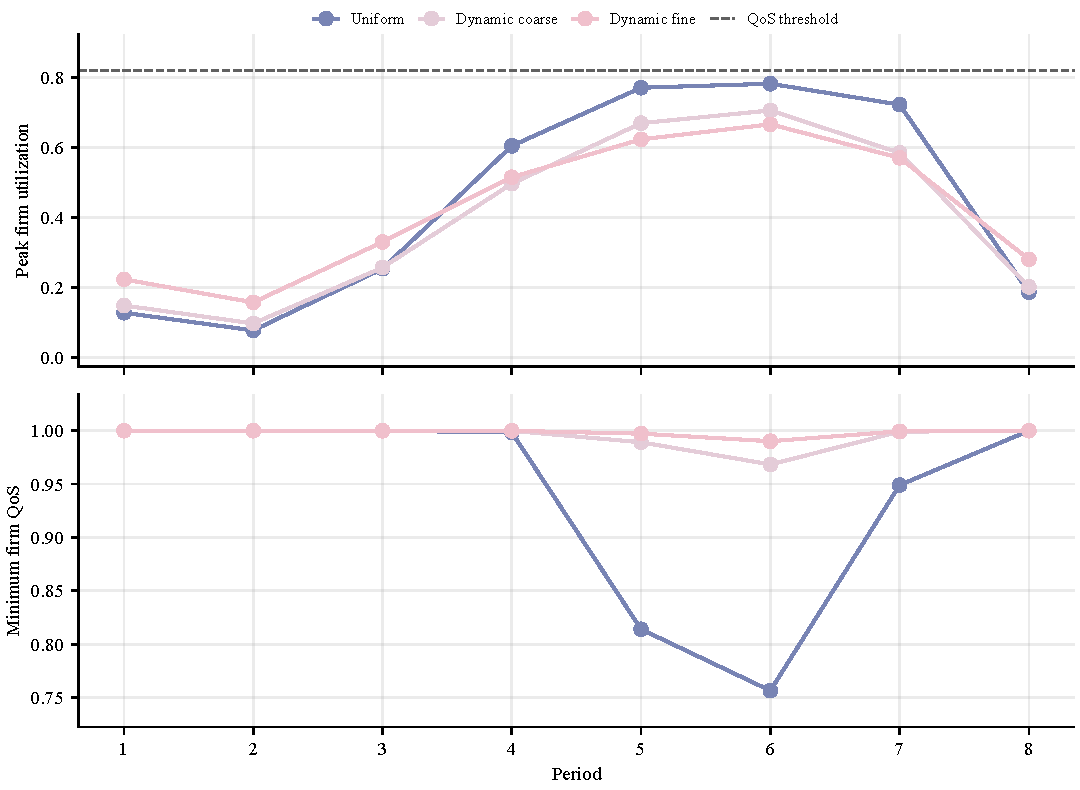
\includegraphics[width=0.86\textwidth]{qos_utilization_profiles.pdf}
\caption{Period-level utilization and QoS in the congested setting. Dynamic pricing lowers peak utilization and raises the worst provider QoS in both coarse and fine snapshots.}
\label{fig:qos_profiles}
\end{figure}

\begin{figure}[H]
\centering
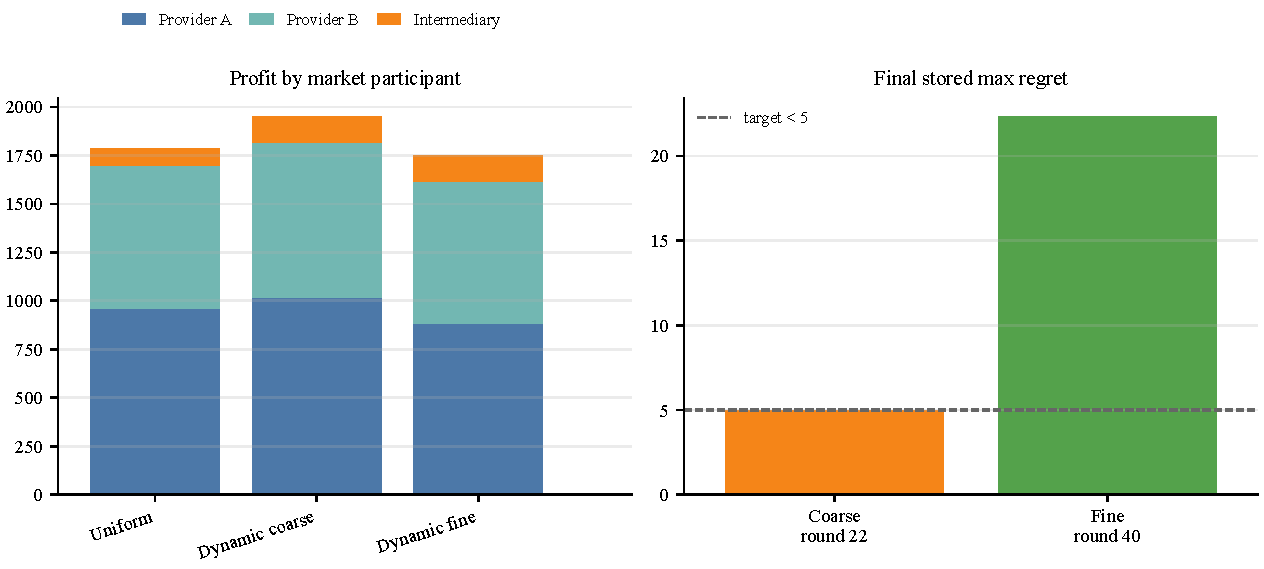
\includegraphics[width=0.88\textwidth]{profit_components_and_regret.pdf}
\caption{Profit components and snapshot regret. The coarse grid reaches regret below 5, whereas the fine-grid pure snapshot remains high-regret after 40 rounds.}
\label{fig:profit_regret}
\end{figure}

\begin{figure}[H]
\centering
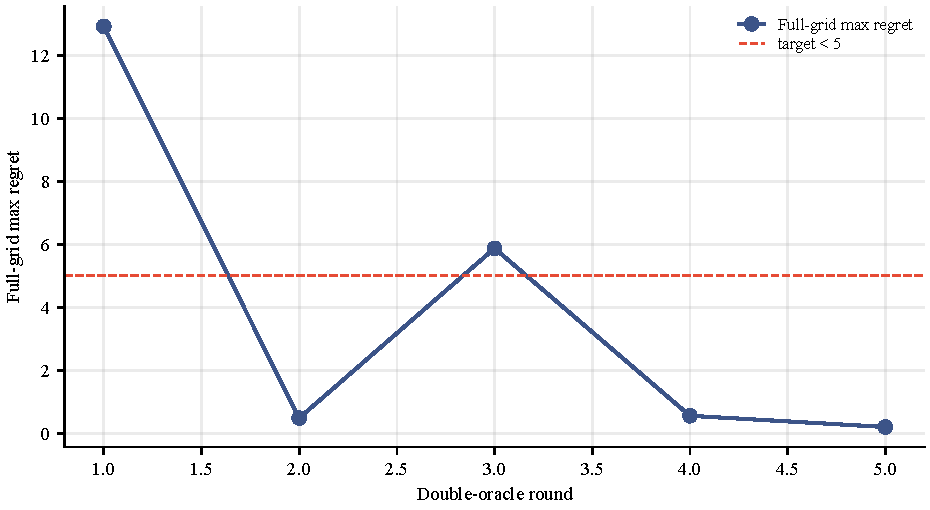
\includegraphics[width=0.76\textwidth]{mixed_oracle_regret.pdf}
\caption{Double-oracle finite-grid mixed-strategy diagnostic. Each round adds best deviations on the full 225-point grid. The final $5\times5$ support profile reaches full-grid maximum regret $0.203$.}
\label{fig:mixed_oracle}
\end{figure}

The QoS direction is stable across the reported objects. Uniform pricing reaches minimum QoS $0.756$ and peak utilization $0.782$. The dynamic snapshots reduce peak utilization to the $0.66$--$0.71$ range and raise minimum QoS to the $0.97$--$0.99$ range. The low-regret finite-grid mixed profile has expected peak utilization $0.703$ and minimum QoS $0.970$. The main QoS result is not tied only to the high-regret fine-grid pure snapshot.

The profit result is different. System profit changes from $+9.3\%$ on the coarse grid to $-1.9\%$ for the fine snapshot and about $-2.8\%$ for the mixed profile. We do not treat profit improvement as a positive finding. The supported reading is narrower: time-of-use pricing protects QoS in the congested fixed-capacity setting, but the current evidence does not show a reliable profit gain.

The provider-heterogeneity hypothesis is also not stable. One might expect the smaller provider to use stronger dynamic pricing, but the direction changes with grid resolution. The coarse grid gives $\delta_A=0.383$ and $\delta_B=0.023$; the fine grid gives $\delta_A=0.059$ and $\delta_B=0.278$. The paper drops any claim about which provider becomes more dynamic.

\subsection{SMPT baseline diagnostics}

To address the risk that uniform pricing is too weak a baseline, we add four service-management diagnostics around the congested setting: off-peak discount only, peak surcharge only, dynamic coarse pricing with fixed equal routing, and an admission-control diagnostic. Table~\ref{tab:smpt_baselines} reports these baselines next to the static candidate response and the two reported dynamic snapshots.

\begin{table}[H]
\centering
\caption{SMPT baseline diagnostics in the congested setting}
\label{tab:smpt_baselines}
\small
\begin{tabular}{lcccc}
\toprule
Policy or diagnostic & Peak util. & Min QoS & Profit change & Served volume \\
\midrule
Static pricing with QoS routing & 0.782 & 0.756 & -- & 2610 \\
Off-peak discount only & 0.766 & 0.833 & $+5.0\%$ & 2849 \\
Peak surcharge only & 0.738 & 0.921 & $+5.8\%$ & 2672 \\
Dynamic coarse & 0.706 & 0.968 & $+9.3\%$ & 2865 \\
Dynamic fine snapshot & 0.666 & 0.990 & $-1.9\%$ & 3043 \\
Dynamic coarse with equal routing & 0.753 & 0.881 & $+5.9\%$ & 2817 \\
\bottomrule
\end{tabular}
\end{table}

The one-sided price-shape baselines improve QoS, but they do not match the full dynamic coarse snapshot. Off-peak discounts increase served volume but leave more peak pressure than the full dynamic shape. Peak surcharges reduce peak utilization more directly but recover less served volume. Equal routing still improves on the static baseline, yet it leaves minimum QoS at $0.881$ rather than $0.968$, which indicates that both price timing and QoS-aware routing matter. Matching the dynamic coarse peak utilization with a uniform-price admission-control diagnostic would require admitting as little as $90.2\%$ of demand in the tightest period and $97.4\%$ on average; this diagnostic is not a profit comparison, but it shows the service-quality cost of achieving a similar peak-utilization target by throttling rather than pricing.

\subsection{Structural ablations and re-solved sensitivity}

The structural ablations are intentionally small. Removing the outside option, suppressing the direct-provider channel, equalizing provider capacities, removing time-flexible users, and fixing equal routing test whether the QoS result is tied to a single modelling component. The dynamic coarse policy keeps a material positive QoS gain in four ablation rows. Two boundary cases are informative: suppressing the direct-provider channel makes both policies nearly uncongested, so the dynamic advantage almost disappears; equalizing provider capacity reverses the dynamic coarse advantage, with QoS gain $-0.054$ and profit change $-3.6\%$. This narrows the claim. The observed QoS protection is strongest when the market has heterogeneous capacity, direct/provider alternatives, and congestion severe enough for prices to matter.

\subsection{Local parameter stress tests}

To check whether the QoS direction is tied to one synthetic calibration, we evaluate the reported uniform, dynamic coarse, and dynamic fine policies under nine local perturbations. The perturbations cover capacity scale, price sensitivity, switching cost, and the QoS threshold. These are fixed-policy stress tests. They are not equilibrium re-solves at each parameter point.

\begin{figure}[H]
\centering
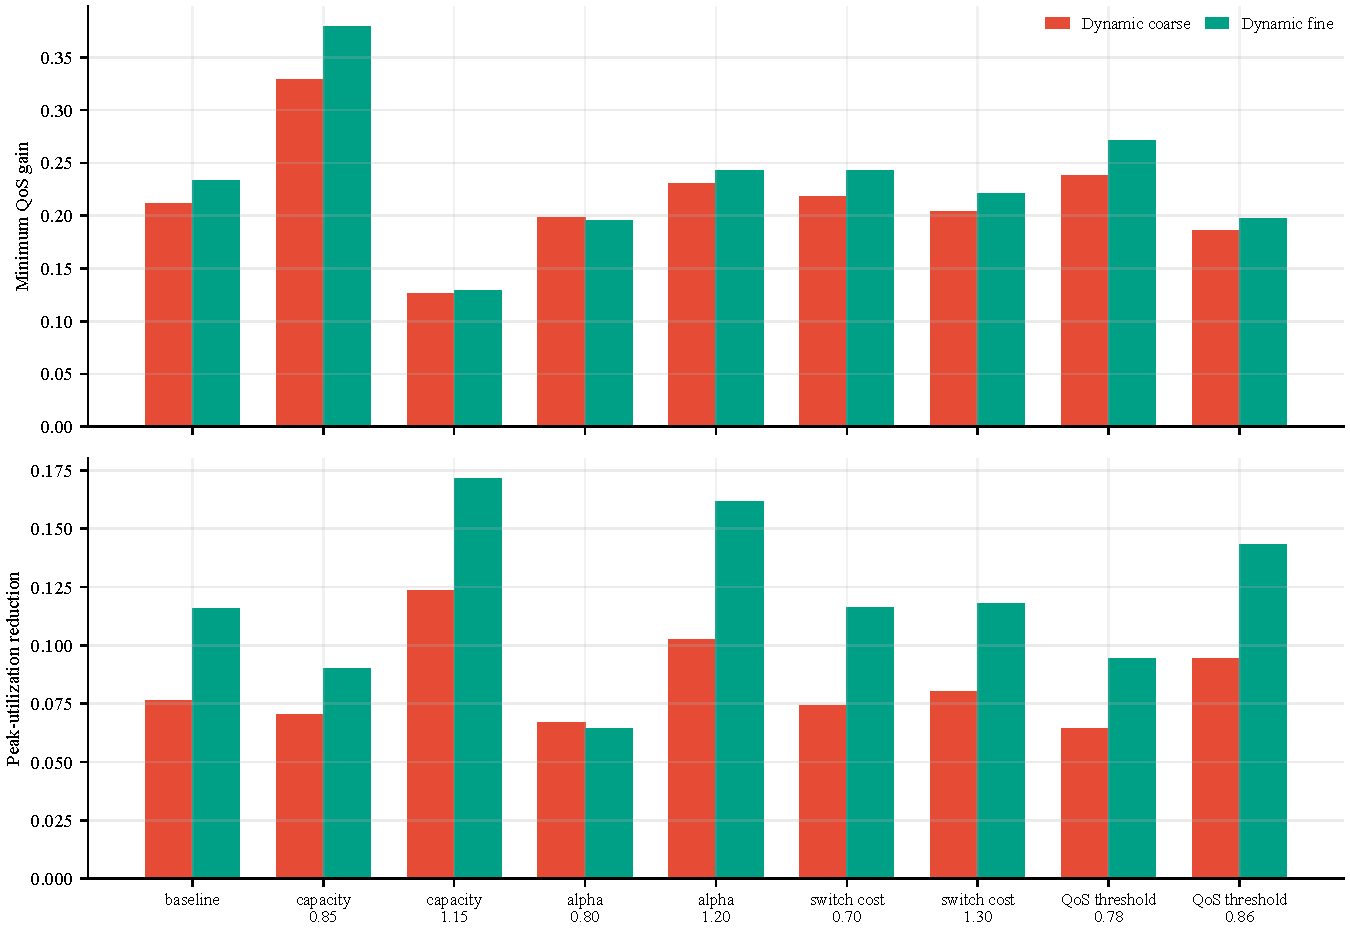
\includegraphics[width=0.92\textwidth]{parameter_sweep_qos.pdf}
\caption{Local parameter stress tests. Across nine perturbation scenarios, both dynamic snapshots keep positive minimum-QoS gains and positive peak-utilization reductions relative to uniform pricing.}
\label{fig:parameter_sweep}
\end{figure}

Both dynamic snapshots keep positive QoS gains and lower peak utilization in all nine perturbation scenarios. The smallest minimum-QoS gain is $0.126$ for the coarse snapshot and $0.129$ for the fine snapshot. Profit remains unstable: the coarse snapshot is positive in all nine scenarios, while the fine snapshot is positive in only one. This reinforces the QoS result while keeping the profit conclusion modest.

\begin{figure}[H]
\centering
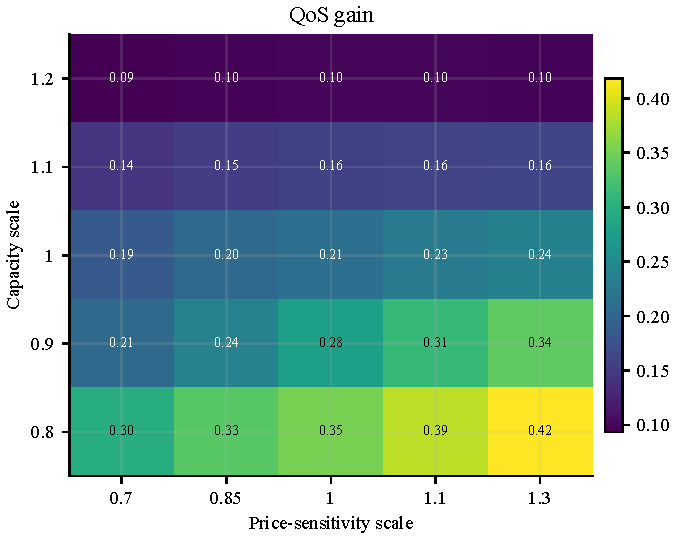
\includegraphics[width=0.48\textwidth]{smpt_phase_qos_gain.pdf}
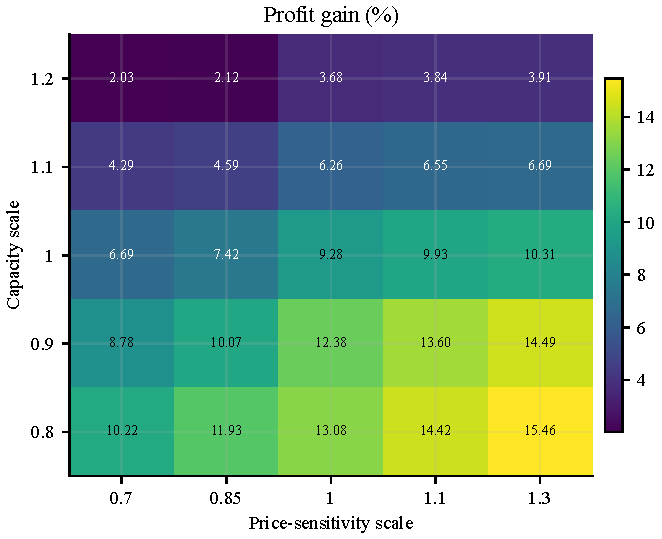
\includegraphics[width=0.48\textwidth]{smpt_phase_profit_gain.pdf}
\caption{Fixed-policy phase grid over capacity scale and price-sensitivity scale. The dynamic coarse policy keeps positive QoS gains and peak-utilization reductions in all 25 grid points; profit is positive on this fixed-policy grid, but the restricted re-solved sensitivity below remains mixed.}
\label{fig:smpt_phase}
\end{figure}

The fixed-policy phase grid gives a broader local view: QoS gain and peak-utilization reduction are positive in all 25 capacity--elasticity grid points, with minimum QoS gain $0.094$. Profit is positive on this fixed-policy coarse-policy grid, ranging from $+2.0\%$ to $+15.5\%$. This does not overturn the profit-boundary result, because it keeps the coarse policy fixed.

For a stronger check, we re-solve a restricted local candidate set at five perturbation points. The candidate set contains the static, dynamic coarse, dynamic fine, off-peak-only, and peak-only shapes, and each scenario runs four local best-response rounds. The re-solved rows keep positive QoS gain in all five cases, with gains between $0.156$ and $0.280$. Profit remains mixed: capacity tightening and a lower QoS threshold give $+12.5\%$ and $+11.0\%$, while higher price sensitivity and a larger flexible-user share give $-1.4\%$ and $-1.9\%$. This is the strongest current evidence for the paper's central separation: QoS protection is easier to reproduce than profit improvement.

\section{Mechanism and Profit-Boundary Discussion}
\label{sec:discussion}

The main empirical pattern is not subtle. QoS improves sharply in the congested setting, but profit does not improve reliably. The reason is that time-of-use pricing reallocates demand; it does not create additional GPU supply.

\begin{figure}[H]
\centering
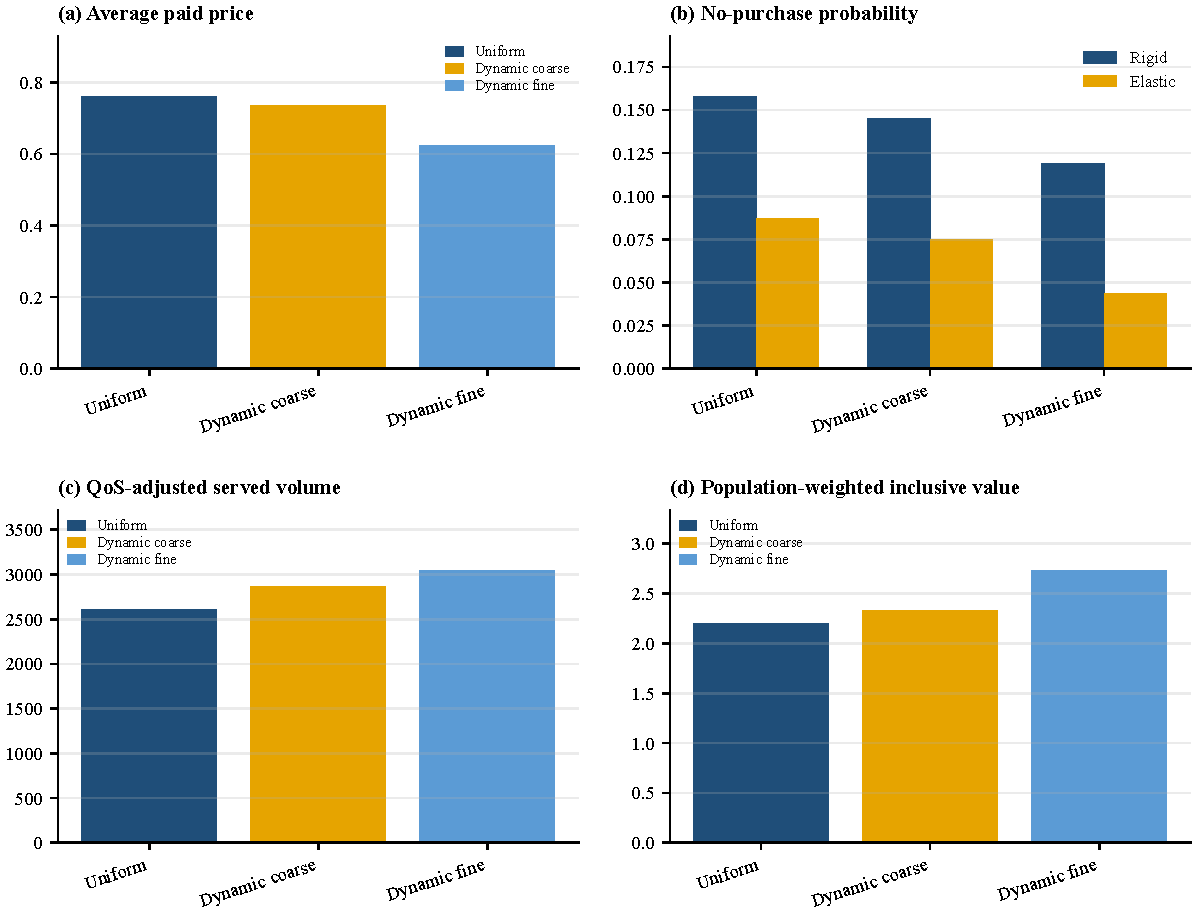
\includegraphics[width=0.9\textwidth]{mechanism_diagnostics.pdf}
\caption{Mechanism diagnostics. Dynamic pricing raises QoS-adjusted served volume and lowers exit probabilities, while the average paid price falls. The improvement is closer to coverage and reliability than to a stable profit gain.}
\label{fig:mechanism}
\end{figure}

Figure~\ref{fig:mechanism} shows the relevant accounting. Under uniform pricing, QoS-adjusted served volume is $2610$. Under the dynamic coarse and fine snapshots, it rises to $2865$ and $3043$. Rigid-user exit falls from $0.158$ to $0.145/0.119$, and flexible-user exit falls from $0.087$ to $0.075/0.044$. Dynamic pricing recovers some service volume that congestion would otherwise destroy.

That recovery does not automatically become profit. The average paid price falls from $0.761$ to $0.735/0.625$. Peak-period price increases can improve margins, but they also push price-sensitive demand toward the rival provider, the direct channel, or the outside option. Off-peak discounts use idle capacity, but they thin per-request margins. The mixed profile suggests that these opposing forces can leave providers with better QoS and no stable profit gain.

This is not a fixed-total-demand theorem. The model allows users to exit and allows market size to expand at lower prices. A better description is surplus reallocation. Prices move demand across time and channels, and some of the recovered congestion loss shows up as better completion and lower exit rather than as provider profit.

For operators, the lesson is practical. Time-of-use pricing should not be sold as a dependable revenue lever under fixed capacity and competition. It is more defensible as a service-quality tool: a way to reduce peak overload, improve completion, and protect SLA-like metrics. For regulators or platform designers, the same point matters in reverse. A higher peak price is not automatically evidence of extraction if it also reduces failed service. The welfare question depends on prices, completion, exit, and user surplus together.

\section{Limitations}
\label{sec:limitations}

The main limitation is calibration. Price sensitivity, switching cost, capacity cost, population mix, and outside-option utility are synthetic. The numerical percentages in the paper should be read as mechanism evidence, not production forecasts. Public API prices give only a price-scale reference. The controlled vLLM scans give only a QoS-shape reference under a single GPU, small models, short generations, and a small set of concurrency levels.

The solver evidence is also bounded. Provider strategies are restricted to a low-dimensional pricing-shape family. The fine-grid pure snapshot remains high-regret, and the double-oracle mixed profile lowers regret only on the finite 225-point candidate grid. The phase grid evaluates fixed policies under perturbations, and the re-solved sensitivity uses a restricted local candidate set rather than a full re-optimization at each point. These choices are acceptable for an auditable simulation paper, but they should not be read as a continuous-space equilibrium proof or global uncertainty quantification.

The market structure is intentionally small. The model has two providers and one API intermediary. Many-provider competition, multiple intermediaries, long-term capacity contracts, differentiated model quality, and dynamic capacity procurement are left outside the current scope. Real deployment would require request traces, context-length distributions, production completion curves, user elasticity estimates, and online experiments.

\section{Conclusion}
\label{sec:conclusion}

This paper asked whether time-of-use dynamic pricing can protect inference-service QoS when GPU serving capacity is fixed. In the congested synthetic setting, the answer is yes in a bounded finite-grid sense. Dynamic pricing lowers peak utilization and raises the minimum QoS, and a double-oracle mixed-strategy diagnostic reduces full-grid regret to $0.203$ on the 225-point candidate grid. Local fixed-policy perturbations preserve the same QoS direction.

The profit result is less favorable and more useful than a simple positive story. Profit changes sign across solver objects, and the low-regret mixed profile is negative relative to uniform pricing. The evidence points to surplus reallocation: time-of-use prices recover some congestion loss and reduce exit, but competition, discounts, and outside options prevent that gain from reliably becoming provider profit. The paper's contribution is a reproducible way to see this QoS-profit separation under fixed capacity, not a claim that dynamic pricing is a universal revenue-improvement tool.

\section*{Reproducibility, Data Availability, and Artifact Boundary}

The peak-shaving simulation modules are \path{pricing_sim/peak_shaving_config.py},
\path{pricing_sim/peak_shaving_market.py}, and
\path{pricing_sim/peak_shaving_equilibrium.py}. The main experiment entry points are:
\begin{itemize}[leftmargin=2em]
  \item \path{experiments/run_peak_shaving_experiments.py}: uncongested main experiment;
  \item \path{experiments/run_peak_shaving_congested_fp.py}: congested fictitious play;
  \item \path{experiments/run_fp_dynamic_converge.py}: regret convergence and checkpoint continuation;
  \item \path{experiments/run_peak_shaving_robustness.py}: QoS-shape, outside-option, and cross-seed checks;
  \item \path{experiments/run_peak_shaving_mixed_oracle.py}: finite-grid mixed-strategy diagnostic;
  \item \path{experiments/run_peak_shaving_parameter_sweep.py}: local parameter stress tests;
  \item \path{experiments/run_peak_shaving_smpt_experiments.py}: SMPT baselines, ablations, phase grid, restricted local re-solve, and fixed-point residual diagnostics;
  \item \path{experiments/run_peak_shaving_smpt_vv_audit.py}: initial-condition and damping-factor fixed-point audit;
  \item \path{experiments/build_peak_shaving_measurement_anchor.py}: controlled vLLM QoS-shape anchor.
\end{itemize}
Machine-readable artifacts are under \path{artifacts/peak_shaving/}, with the main subdirectories
\path{20260618/}, \path{20260619/}, \path{20260619_submission/}, and \path{20260619_smpt/}. Figures are under
\path{figures/peak_shaving_diagnostics/}, \path{figures/peak_shaving_submission/}, and \path{figures/peak_shaving_smpt/}. Parameter tables,
grid definitions, artifact mappings, and reproduction commands are provided in
\path{peak_shaving_dynamic_pricing_sci_en_supplement_2026-06-19.tex}.

The current artifact package is available in the public repository \url{https://github.com/cccht/paper_token_price}. A formal submission should cite a frozen release or archival DOI for the code, configuration files, raw JSON/CSV artifacts, figure scripts, and generated figures. Until that archival release is created, the GitHub repository should be treated as a living reproducibility package rather than a persistent data identifier.

\section*{Declaration of Generative AI and AI-Assisted Technologies}

AI-assisted tools were used during manuscript preparation for language editing, structural checking, and pre-submission review simulation. The authors reviewed and edited the resulting text and take responsibility for the content of the manuscript.

\small
\bibliographystyle{unsrtnat}
\bibliography{verified_refs}

\end{document}
